% Plantilla para Trabajos Finales en la EPEF (UDC)
\documentclass{Plantilla/Formato_EPEF}

% Los paquetes están incluidos en la plantilla, no en este documento

%%%%%%%%%%%%%%%%%%%%%%%%%%%%%
% Datos relativos al alumno %
%%%%%%%%%%%%%%%%%%%%%%%%%%%%%
% Nombre del autor del trabajo
\newcommand{\Autor}{Francisco Rodríguez Gavín}
% Sexo del autor (comentar el que no sea correcto)
\newcommand{\AutorSex}{Autor}
%\newcommand{\AutorSex}{Autora}
% Titulación para la que se presenta el Trabajo Final (comentar el que no sea correcto)
%\newcommand{\Titulacion}{Elegir la titulación correspondiente}
% \newcommand{\Titulacion}{Grado Dual en Ingeniería Eléctrica}
% \newcommand{\Titulacion}{Grado en Ingeniería Electrónica Industrial y Automática}
% \newcommand{\Titulacion}{Grado Abierto en Ingeniería Industrial}
% \newcommand{\Titulacion}{Grado en Ingeniería en Tecnologías Industriales}
%\newcommand{\Titulacion}{Grado en Ingeniería Mecánica}
% \newcommand{\Titulacion}{Grado en Ingeniería Naval y Oceánica}
%\newcommand{\Titulacion}{M. U. en Eficiencia Energética y Sostenibilidad}
% \newcommand{\Titulacion}{M. U. en Informática Industrial y Robótica}
% \newcommand{\Titulacion}{M. U. en Diseño, Desarrollo y Comercialización de Videojuegos}
 \newcommand{\Titulacion}{M. U. en Ingeniería Industrial}
% \newcommand{\Titulacion}{M. U. en Ingeniería Naval y Oceánica}
% \newcommand{\Titulacion}{M. U. en Materiales Complejos: Análisis Térmico y Reología}
% \newcommand{\Titulacion}{M. U. en Erasmus Mundus en Sostenibilidad e Industria 4.0 aplicada al Sector Marítimo}
% Nombre de la escuela
\newcommand{\Escuela}{Escuela Politécnica de Ingeniería de Ferrol}
\newcommand{\EscuelaAbrevidado}{EPEF}
% Dirección de la escuela
\newcommand{\Direccion}{Rúa Mendizábal, s/n, Campus de Esteiro, 15403, Ferrol}

%%%%%%%%%%%%%%%%%%%%%%%%%%%%%%%%%%%%
% Datos relativos al Trabajo Final %
%%%%%%%%%%%%%%%%%%%%%%%%%%%%%%%%%%%%
% Título del Trabajo Final
\newcommand{\TituloUno}{Diseño de una instalación fotovoltaica de autoconsumo}
\newcommand{\TituloDos}{} % Usar sólo si el título es demasiado largo
%\newcommand{\TituloTres}{} % Usar sólo si el título es demasiado largo
% Número asociado al Trabajo Final
%\newcommand{\Numero}{2324\_GEM\_30}
% Tipo de Trabajo Final (comentar el que no sea correcto)
\newcommand{\TipoTrabajo}{Instalaciones Eléctricas}
\newcommand{\TipoAbreviado}{Instalación FV}
%\newcommand{\TipoTrabajo}{Trabajo Fin de Máster}
%\newcommand{\TipoAbreviado}{TFM}
% Tutor/es (en caso de no haber co-tutor, se deberá de comentar la línea correspondiente)
\newcommand{\TutorUno}{Antonio Enrique Masdías Bonome}
%\newcommand{\TutorDos}{} % Usar sólo en caso de haber un co-tutor
% Sexo y número del tutor (comentar el que no sea correcto)
\newcommand{\TutorSex}{Tutor}
%\newcommand{\TutorSex}{Tutora}
%\newcommand{\TutorSex}{Tutores}
%\newcommand{\TutorSex}{Tutoras}
% Fecha de presentación del Trabajo Final
\newcommand{\Fecha}{Enero de 2026}
%\newcommand{\FechaAbreviada}{Sept. 2025}
\newcommand{\Curso}{2025/2026}

\usepackage{comment}
\usepackage{arydshln}
\usepackage[T1]{fontenc}
\usepackage{siunitx}

\makeatletter
\addto\captionsspanish{\renewcommand{\contentsname}{Índice}}
\makeatother


\renewcommand{\thesection}{\arabic{section}}

\begin{document}
\subfile{Plantilla/Portada_principal}
%\subfile{Plantilla/Portada_documento}
%\vspace*{-1.5cm}

% --- CORRECCIÓN ---
% 1. Cambiamos la variable interna de la plantilla para el pie de página
\renewcommand{\NombreDocumento}{Índice} 

% 2. Aseguramos que el título de la página también sea correcto (por si babel molesta)
\renewcommand{\contentsname}{Índice}

\tableofcontents
\newpage

\renewcommand{\NombreDocumento}{Introducción}

\section{Introducción}

Se desea proyectar la instalación eléctrica de una vivienda unifamiliar de grado elevado con los siguientes circuitos especiales, además de los mínimos establecidos en el REBT (ver figura \ref{Enunciado_1}):
\begin{itemize}
	\item Circuito de alumbrado exterior: \SI{800}{W}.
	\item Cargador de vehículo eléctrico de \SI{7}{kW} de la marca V2C.
	\item Instalación de autoconsumo formada por:
	\begin{itemize}
		\item Línea a inversor de \SI{25}{m} de longitud.
		\item Inversor fotovoltaico (FV) monofásico de \SI{6}{kW} \textit{Fronius Gen 24 6.0 Plus}.
		\item Campo Solar FV situado a 38 metros de distancia del inversor equipado con 10 paneles solares \textit{Canadian Solar Hiku7 CS/N-665MS}.
	\end{itemize}
	
	\item La Derivación Individual (DI) dispone de una distancia de 30 metros entre la CGPM y el Cuadro General de la vivienda.
\end{itemize}


\begin{figure}[!ht]
	\centering
	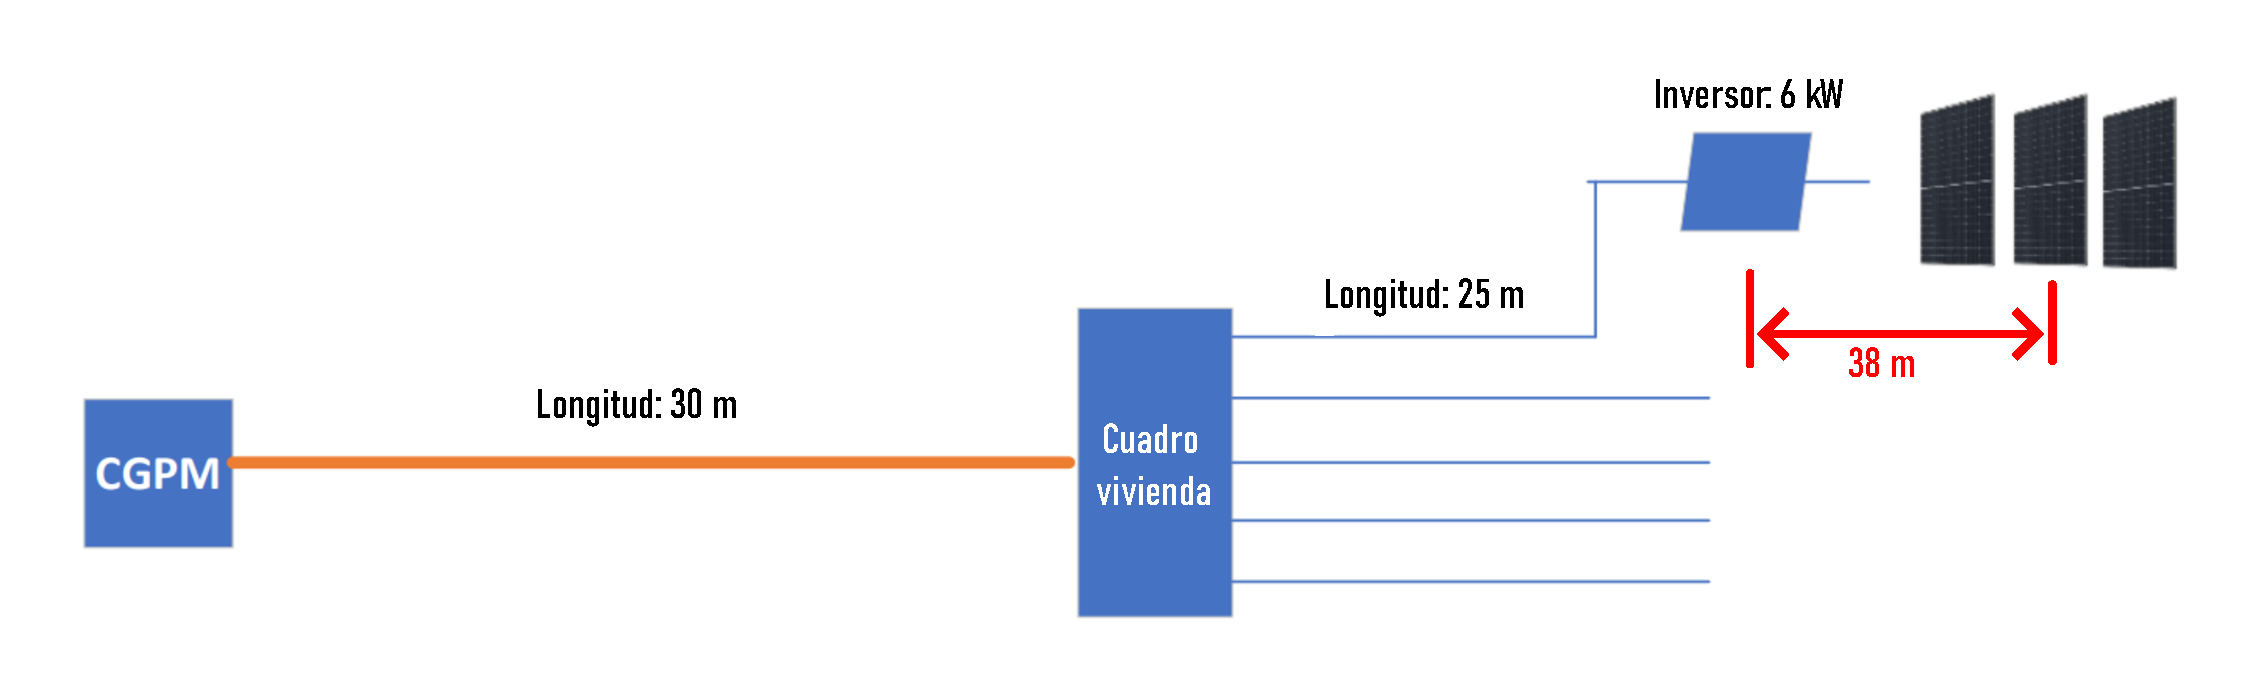
\includegraphics[width=1\textwidth]{Figuras/Enunciado_1.pdf}
	\caption{Esquema de la instalación eléctrica a diseñar}
	\label{Enunciado_1}
\end{figure}

\subsection{Características técnicas inversor}
Las características del inversor monofásico FV son las siguientes:

\textbf{Datos de entrada}
\begin{itemize}
	\item Número de seguidores MPP: 2
	\item Rango de tensión de entrada CC: 65 - 600 V.
	\item Rango de tensión MPP: 65 - 480 V.
	\item Número de entradas CC: 2 (MPPT1 y MPPT2)
	\item Máxima corriente de entrada por MPP:
	\begin{itemize}
		\item MPPT1: 22 A.
		\item MPPT2: 12 A.
	\end{itemize}
	\item Máxima potencia en CC:
	\begin{itemize}
		\item MPPT1: 6200 W.
		\item MPPT2: 5760 W.
	\end{itemize}
	\item Potencia pico del generador FV:
	\begin{itemize}
		\item MPPT1: 7500 W.
		\item MPPT2: 5760 W.
	\end{itemize}
\end{itemize}

\textbf{Datos de salida}
\begin{itemize}
	\item Potencia nominal CA: 6000 W.
	\item Voltaje de salida: 230 V.
	\item Corriente de salida CA nominal: 26,1 A.
	\item Frecuencia: 50/60 Hz.
	\item Factor de potencia: 0,8 - 1 ind./cap.
\end{itemize}

\subsection{Características técnicas de los paneles solares}\label{Caract_panel}
Por otro lado, las características técnicas más relevantes de los paneles solares \textit{Canadian Solar Hiku7 CS/N-665MS} que componen la instalación fotovoltaica, son las siguientes:
\begin{itemize}
	\item Potencia nominal máxima por panel ($P_{max}$): 665 W.
	\item Voltaje de operación por panel ($V_{mp}$): 38,5 V.
	\item Corriente de operación ($I_{mp}$): 17,28 A.
	\item Voltaje de circuito abierto ($V_{op}$): 45,6 V.
	\item Intensidad de cortocircuito ($I_{sc}$): 18,51 A.
	\item Dimensión de los paneles: 2384x1303x35 mm.
\end{itemize}


\section{Esquema eléctrico de la instalación}
\renewcommand{\NombreDocumento}{Esquema eléctrico de la instalación}

De acuerdo con el apartado \textit{2.Clasificación} de la \textit{ITC-BT-40}, en el presente proyecto se tiene una instalación generadora interconectada para autoconsumo con excedentes, de manera que si existe una demanda en la vivienda menor que la producida por la instalación fotovoltaica, el excedente se volcará a la red.

De acuerdo con la \textit{Guía ITC-BT-40}, se establece que la instalación del presente proyecto tiene la categoría \textit{C1}:

\textit{\textgravedbl Instalaciones generadoras con punto de conexión en la red de distribución de baja tensión en la que hay otros circuitos e instalaciones de baja tensión conectados a ella, independientemente de que la finalidad de la instalación sea tanto vender energía como alimentar cargas, en paralelo con la red\textacutedbl}.

En este tipo de instalaciones, se considera que las instalaciones de conexión entre una instalación generadora y la red comienzan en la Caja General de Protección y Medida (CGPM), y terminan en los dispositivos generales de mando y protección de la instalación fotovoltaica generadora.

De acuerdo con la información aportada en el enunciado, el esquema de la instalación que se proyectará será el \textit{Esquema 8} de la \textit{Guía ITC-BT-40}. En dicho esquema, se refleja que el circuito de la parte de generación de la instalación, es independiente de la instalación eléctrica de consumo, y este parte de Cuadro de Mando y Protección (CMP) de la vivienda unifamiliar (figura \ref{Esquema_8}).

\begin{figure}[!ht]
	\centering
	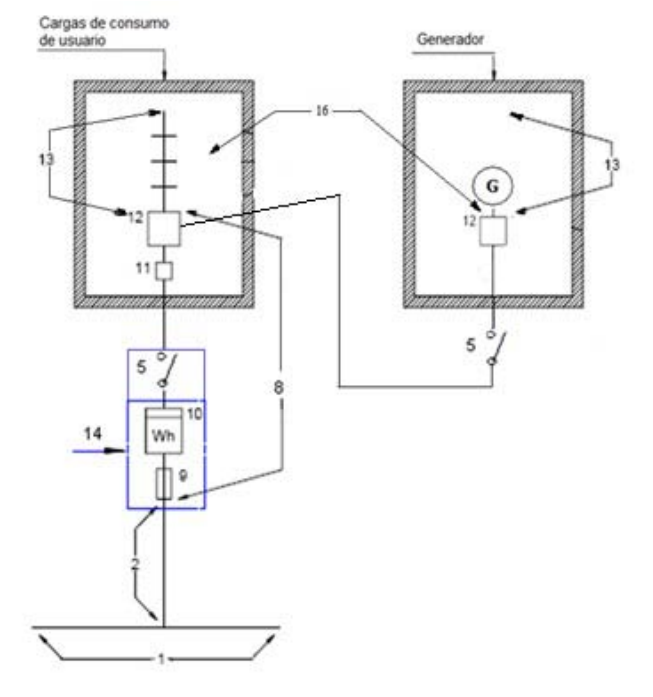
\includegraphics[width=0.7\textwidth]{Figuras/Esquema_8.png}
	\caption{Esquema 8 de la \textit{Guía ITC-BT-40}}
	\label{Esquema_8}
\end{figure}


De acuerdo con lo que observa en el esquema de la instalación, no existe una LGA como tal, ya que se trata de un vivienda unifamiliar, por lo que después de la CGPM se tiene la Derivación Individual (DI). Además, será necesario el uso de un contador bidireccional, ya que se trata de una instalación con generación para autoconsumo con excedentes.

Por otro lado, tal y como se especifica en el enunciado, se tienen 3 tipos de circuitos: 1 circuito de generación que se corresponde con las instalaciones de producción de energía eléctrica fotovoltaica, y 2 circuitos de consumo (VE y alumbrado exterior). Se realizará el diseño de la derivación individual (DI) y del circuito de generación. Para los dos circuitos de consumo no se puede realizar un diseño de los conductores, ya que se desconoce su longitud.

\section{Instalación de generación fotovoltaica}
\renewcommand{\NombreDocumento}{Instalación de generación fotovoltaica}
Esta instalación tiene dos partes diferenciadas, una correspondiente a la parte de corriente continua (CC) que se encuentra entre el inversor y los paneles solares, y otra que es de corriente alterna (CA) y que se sitúa entre el inversor y CMP de la vivienda.

\subsection{Instalación de CC}
Teniendo en cuenta las características técnicas de los paneles solares descritas en el apartado \ref{Caract_panel}, se tiene que al ser una instalación de generación FV compuesta por 10 paneles colocados en serie, la tensión total de operación entre bornes ($V_{t,FV}$) es de:

\begin{equation}
	V_{t,FV} = 10 \cdot V_{mp} = 10 \cdot \SI{38,5}{V} = \SI{385}{V}
\end{equation}

Además, siguiendo la misma lógica, el voltaje total en circuito abierto ($V_{t,op}$) será igual a 456 V.

A continuación, hay que comprobar que el inversor monofásico que se ha propuesto, tiene un rango de tensión de entrada lo suficientemente elevado, para soportar la tensión que le otorgará la instalación FV. Realizando dicha comprobación, se concluye que el inversor sí es válido porque su rango de tensión de entrada llega hasta los 600 V y $V_{t,op}$ es igual a 456 V, por lo el inversor aguantará el voltaje que como mucho le podrían dar los paneles. Además, el inversor tiene dos entradas CC, siendo la única válida la entrada \textbf{MPPT1}, ya que la corriente de operación ($I_{mp}$) es igual a 17,28 A. Además, esta entrada podrá soportar el voltaje de operación $V_{t,FV}$ de la instalación (385 V < 480 V).


En consecuencia, teniendo en cuenta que cada panel puede llegar a producir 665 W, se tiene que la potencia total que la instalación FV puede llegar a generar ($P_{t,FV}$) es de:

\begin{equation}
	P_{t,FV} = 10 \cdot 665 = \SI{6650}{W}
\end{equation}

No obstante, teniendo en cuenta que la entrada MPPT1 solo puede manejar como mucho 6200 W, este valor es el que realmente entrará en el inversor.

\subsubsection{Dimensionamiento del cable}
Teniendo en cuenta que la distancia entre el inversor y la instalación de paneles fotovoltaicos es de 38 metros, y suponiendo que todos los paneles están colocados en línea, se puede calcular la longitud de cálculo ($L_c$) del cable CC de la siguiente manera:
\begin{equation}
	L_c = 38 + \frac{10\cdot1,303}{2} \simeq \SI{44,5}{m}
\end{equation}

Suponiendo el uso del cable \textbf{TOPSOLAR PV H1Z2Z2-K}, la compañía TOP CABLE da un valor de intensidad máxima admisible ($I_z$) considerando una temperatura inicial de 60\textcelsius. Como se desconoce la temperatura de funcionamiento y la conductividad del cobre a dicha temperatura, se va a realizar una suposición inicial que es considerar que el cable se encuentra a 20\textcelsius. Para esta temperatura el cobre tiene una conductividad de $\SI{56}{m/\Omega\cdot mm^2}$ y a continuación, se calcula la sección de cable necesaria para que haya una caída de tensión de como mucho un \SI{1,5}{\%} (caída de tensión recomendable):
 
\begin{equation}
	S = \frac{2\cdot6200\cdot 44,5}{56\cdot0,015\cdot385\cdot385} = \SI{4,43}{mm^2}
\end{equation}

Por lo tanto, se necesitaría una sección de  $\SI{6}{mm^2}$ para que se cumpla la caída de tensión que se ha propuesto, para una temperatura del cable igual a 20\textcelsius. No obstante, si se supone una temperatura inicial de operación de 60\textcelsius, de acuerdo con los datos otorgados por TOP CABLE, la intensidad máxima admisible es de 70 amperios para dicha sección (ver figura \ref{Intensidad}).

\begin{figure}[!ht]
	\centering
	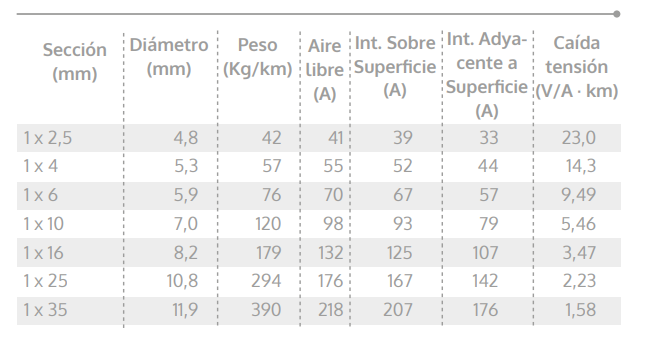
\includegraphics[width=0.7\textwidth]{Figuras/Seccion_topcable.png}
	\caption{Intensidades máximas admisibles a 60\textcelsius}
	\label{Intensidad}
\end{figure}

Además, con respecto a la intensidad nominal ($I_n$), según el apartado \textit{5.Cables de conexión} de la \textit{ITC-BT-40}, se deberán dimensionar los cables de conexión entre la generación y el inversor para una intensidad mínima del orden del 125\% de la máxima intensidad del generador, es decir, la intensidad de cortocircuito de la instalación fotovoltaica ($I_{sc}$). Por ello, la corriente máxima admisible de los cables de corriente continua tendrá que ser mayor que:
\begin{equation}
	I_{n,cc} = 1,25 \cdot \SI{18,51}{A} = \SI{23,14}{A}
\end{equation}


Ahora que ya se tienen todos los datos, para calcular la temperatura de trabajo ($\theta$) se empleará la siguiente fórmula:
\begin{equation}
	\theta = T_0 + (T_{max}-T_0)\cdot\left(\frac{I_c}{I_z}\right)^2 = 60 + (120 - 60)\cdot\left(\frac{23,14}{70}\right)^2 = \SI{66,56}{C}
\end{equation}

Para calcular la conductividad térmica del cobre a 66,56 \textcelsius, se emplea la siguiente fórmula:
\begin{equation}
	\sigma_{Cu,66,56} = \frac{1}{\rho_{20}\cdot[1 + \alpha_{20}\cdot(\theta - 20)]} =  \frac{1}{0,018\cdot[1 + 0,00392\cdot(66,56 - 20)]} = \SI{46,98}{m/\Omega\cdot mm^2}
\end{equation}

Calculando de nuevo, con la conductividad del cobre a la temperatura de trabajo, la sección necesaria para cumplir con la caída de tensión:

\begin{equation}
	S_{FV,CC} = \frac{2\cdot6200\cdot 44,5}{46,98\cdot0,015\cdot385\cdot385} = \SI{5,28}{mm^2}
\end{equation}

Por lo tanto, la sección que se necesita es de $\SI{6}{mm^2}$, para la cual se tiene una $I_z$ igual a 70 amperios que es mayor que la intensidad nominal $I_{n,cc}$.

Con respecto a las protecciones, será necesario poner a tierra el marco de la estructura de los paneles solares y también habrá que instalar un sobretensiones de tipo 1 y 2 con el objetivo de proteger al inversor ante posibles de caídas de rayo sobre la instalación fotovoltaica. Además, también se instalará un fusible de 20 A como protección contra sobreintensidades.

\subsection{Instalación de CA}
Para llevar la potencia desde el inveror hasta el cuadro de la vivienda, se propone el uso de conductores de cobre aislados de tensión asignada 450/750 V y aislamiento de PVC. El método de instalación que se propone para el conductor es bajo tubo en montaje superficial (B1) y según el apartado \textit{5.Cables de conexión} en la \textit{ITC-BT-40}, no se puede superar una caída de tensión del \SI{1,5}{\%}. Situándose en el caso más desfavorable y suponiendo una temperatura de trabajo igual a 70\textcelsius, la conductividad del cobre tiene un valor de  $\SI{48}{m/\Omega\cdot mm^2}$. Además, teniendo en cuenta que la potencia máxima que puede otorgar el inversor es de \SI{6}{kW}:
\begin{equation}
	S_{FV,ac} = \frac{2\cdot6000\cdot25 }{48\cdot0,015\cdot230\cdot230} = \SI{7,87}{mm^2}
\end{equation}

De acuerdo con la tabla \textit{C.52.1 bis 1} de la \textit{UNE-HD 60364-5-52:2022}, la sección necesaria será igual $\SI{10}{mm^2}$ y el conductor tendrá una intensidad admisible de 50 A, la cual es superior a la intensidad nominal ($I_{n,ac}$):

\begin{equation}
	I_{n,ac} = \frac{P}{V} = \frac{\SI{6000}{W}}{\SI{230}{V}} \simeq \SI{26,1}{A} < \SI{50}{A}
\end{equation}

Por lo tanto, para la instalación eléctrica interior que va desde el CPM hasta el inversor estará compuesta por unos conductores \textbf{H07Z1-K TYPE 2 (AS)} de $\SI{10}{mm^2}$ de sección, instalados bajo un tubo de diámetro exterior igual a \SI{16}{mm}, de acuerdo con la \textit{Tabla 2} de la \textit{ITC-BT-21}.


Con respecto a las protecciones, según el apartado \textit{4.3 Instalaciones generadoras interconectadas} de la \textit{ITC-BT-40}, todas las instalaciones generadoras de autoconsumo con excedentes que se conecten a instalaciones interiores lo harán a través de un circuito independiente y dedicado desde un cuadro de mando y protección que esté protegida por un \textbf{diferencial} de \textbf{tipo A} de \SI{30}{mA}. Además, también se deberá poner un sobretensiones de tipo 1 y un magnetotérmico de 32 A.


\section{Dimensionamiento de la Derivación Individual}

Debido a que se trata de una vivienda unifamiliar no existe una LGA, sino que se tiene una derivación individual desde la CGPM hasta el CPM de la vivienda. Como en este caso se trata de una vivienda de Electrificación Elevada, se supone una previsión de cargas igual a 9200 W.

\renewcommand{\NombreDocumento}{Dimensionamiento de la Derivación Individual}

Se propone el uso de conductores de cobre aislados de tensión asignada 450/750 V y aislamiento de PVC. El método de instalación para los conductores será bajo tubo en montaje superficial (B1) y según el apartado \textit{3.Cables} en la \textit{ITC-BT-15} no se puede superar una caída de tensión del \SI{1,5}{\%}. Situándose en el caso más desfavorable y suponiendo una temperatura de trabajo igual a 70\textcelsius, la conductividad del cobre tiene un valor de  $\SI{48}{m/\Omega\cdot mm^2}$. Además, teniendo en cuenta que la longitud de la DI es de 30 metros:

\begin{equation}
	S_{DI} = \frac{2\cdot9200\cdot30 }{48\cdot0,015\cdot230\cdot230} = \SI{14,5}{mm^2}
\end{equation}

De acuerdo con la tabla \textit{C.52.1 bis 1} de la \textit{UNE-HD 60364-5-52:2022}, la sección necesaria será igual $\SI{16}{mm^2}$ y el conductor tendrá una intensidad admisible de 66 A, la cual es superior a la intensidad nominal ($I_{n,DI}$):

\begin{equation}
	I_{n,DI} = \frac{\SI{9200}{W}}{\SI{230}{V}} = \SI{40}{A} < \SI{66}{A}
\end{equation}

Por lo tanto, para la instalación eléctrica de la DI que va desde el CGPM hasta el cuadro de la vivienda, estará compuesta por unos conductores \textbf{H07Z1-K TYPE 2 (AS)} de $\SI{16}{mm^2}$ de sección, instalados bajo un tubo de diámetro exterior igual a \SI{32}{mm}, que es el diámetro mínimo que se obliga a instalar según el apartado \textit{2.Instalación} de la \textit{ITC-BT-15}.

\end{document}
